\documentclass[11pt,letter]{article}
\usepackage[top=1.00in, bottom=1.0in, left=1.1in, right=1.1in]{geometry}
\renewcommand{\baselinestretch}{1.6}
\usepackage{graphicx}
\usepackage{natbib}
\usepackage{amsmath}
\usepackage{amssymb} 
\usepackage{lineno}
\usepackage{xr-hyper}
\externaldocument{decsens_supp}
\externaldocument{letters/plosbio_r1/decsens_plosbio1_p2}
\usepackage{hyperref}
\newcommand{\R}[1]{\label{}\linelabel{#1}} % \newcommand{\R}[1]{\label{#1}\linelabel{#1}}
\newcommand{\lr}[1]{line~\lineref{#1}}
\usepackage{setspace}

\def\labelitemi{--}
\parindent=0pt
\begin{document}

\title{A simple explanation for declining temperature sensitivity \\ with warming} % The illusion of declining temperature sensitivity with warming // Sensitivities are not declining with warming OR As climate change accelerates biology, chasing statistical artifacts ensues
\author{E. M. Wolkovich$^{1,a}$,  J. L. Auerbach$^{2}$, C. J. Chamberlain$^{3}$, D. M. Buonaiuto$^{3}$, \\ A. K. Ettinger$^4$, I. Morales-Castilla$^{5}$ \& A. Gelman$^{2}$} 
\date{} %\today
\maketitle
$^1$Forest \& Conservation Sciences, Faculty of Forestry, University of British Columbia, Vancouver, British Columbia, Canada\\
$^2$Department of Statistics, Columbia University, New York, NY 10027, USA\\
$^3$Department of Organismic and Evolutionary Biology, Harvard University, Cambridge, Massachusetts, USA\\
$^4$The Nature Conservancy in Washington, 74 Wall Street, Seattle, WA, USA\\
$^5$Department of Life Sciences, University of Alcal\`a CTRA N-II, KM., 33,600, 28802, Alcal\`a de Henares, Spain\\
$^a$Corresponding author (ORCID: 0000-0001-7653-893X)
\vspace{3ex}

% \emph{Article type}: Letter\\
% \emph{Short title:} Declining temperature sensitivity\\
% \emph{One sentence summary:} Declining temperature sensitivity with warming is the expected outcome of current methods, not evidence of changing biology.
% Observations of global declines in temperature sensitivity of biological events with climate change have been used as evidence of fundamental shifts in underlying biological processes, but may more simply be explained by the statistical methods used to calculate temperature sensitivity. 


% Phones: Auerbach (dept): 212.851.2132, Holbrook Lab: 617.496-3580, Ailene: 781-296-4821, Nacho: 34 672 74 8160, Gelman: 212-851-2142
% Emails:  jla2167@columbia.edu, cchamberlain@g.harvard.edu, dbuonaiuto@g.harvard.edu, ailene.ettinger@tnc.org, ignacio.moralesc@uah.es, gelman@stat.columbia.edu
\newpage
\linenumbers
\begin{abstract} % 140 plus cites
Temperature sensitivity---the magnitude of a biological response per $^{\circ}$C---is a fundamental concept across scientific disciplines, especially biology, where temperature determines the rate of many plant, animal and ecosystem processes. Recently, a growing body of literature in global change biology has found temperature sensitivities decline as temperatures rise \citep{fu2015,gusewell2017,piao2017,dai2019ag}. Such observations have been used to suggest climate change is reshaping biological processes, with major implications for forecasts of future change. Here we present a simple alternative explanation for observed declining sensitivities: the use of linear models to estimate non-linear temperature responses. Corrections for the non-linearity of temperature response in simulated data and long-term phenological data from Europe remove the apparent decline. Our results show that rising temperatures combined with linear estimates based on calendar time produce observations of declining sensitivity---without any shift in the underlying biology. Current methods may thus undermine efforts to identify when and how warming will reshape biological processes.
\end{abstract}
% Recently, a growing body of literature in global change biology has found temperature sensitivities decline as temperatures rise \citep{fu2015,gusewell2017,piao2017,dai2019ag}. These declines are generally attributed to shifts in underlying biological processes caused by warming, yet to date there is no clear evidence of mechanistic changes.

\newpage
\section{Main text} % 981 right now
Climate change has reshaped biological processes around the globe, with shifts in the timing of major life history events (phenology), carbon dynamics and other ecosystem processes \citep{IPCC:2014sm}. With rising temperatures,  a growing body of literature has documented changes in temperature sensitivity---the magnitude of a biological response scaled per $^{\circ}$C. Many studies have found declining responses to temperature in recent decades \citep{fu2015,gusewell2017,piao2017,dai2019ag}, and some have reported more uniform sensitivities across elevation \citep{vitasse2018}, or lower sensitivities in warmer, urban areas \citep{meng2020}.\\

Most studies attribute changes in temperature sensitivity to shifts in underlying biological processes. For example, researchers have suggested weaker temperature sensitivities are evidence of increased light limitation in the tundra \citep{piao2017}, or a decline in the relative importance of warm spring temperatures for spring phenological events (e.g., leafout, insect emergence) in the temperate zone \citep{fu2015,meng2020}, as other environmental triggers (e.g., winter temperatures that determine `chilling') play a larger role. Yet, despite an increase in studies reporting declining or shifting temperature sensitivities, none have provided strong evidence of the biological mechanisms underlying these changes  \citep[e.g.,][]{fu2015,meng2020}. The missing mechanisms may be hidden in the data: environmental factors moderate biological processes in complex ways \citep{chuine2016,gusewell2017}, are strongly correlated in nature \citep[e.g.,][]{fu2015}, and temperature variance shifts over time and space \citep{keenan2019}. \\
%  fundamental science suggests that warm spring temperatures are the main controller of many temperate phenological events (e.g., leafout, insect emergence), but winter temperatures and photoperiod can also determine the timing of events. Thus, an increased role of winter temperatures or photoperiod could explain observed declines in the temperature sensitivity of plant phenology with warming. 
% ... fundamental science predicts declines in the temperature sensitivity of temperate plant phenology, as the role of spring temperature diminishes relative to the increasing importance of winter temperatures and daylength... For example, the temperature sensitivity of spring leafout may decline if warmer winters mean plants fail to receive enough winter chilling.  

Here we propose a simpler alternative explanation: the use of linear models for non-linear responses to temperature. Researchers generally use methods with assumptions of linearity to calculate temperature sensitivities, often relying on some form of linear regression to compute a change in a quantity---days to leafout or carbon sequestered over a fixed time, for example---per $^{\circ}$C, thus ignoring that many biological responses to temperature are non-linear. We show, theoretically then with simulated and empirical data, how the use of linear methods for non-linear responses\R{semantic1} can produce an illusion that the mechanisms underlying biological processes are changing.\\ % We demonstrate this theoretically using first-hitting-time models---and empirically---using both simulated data and long-term phenological data from Europe.\\

Many observed biological responses\R{semantic2} are the result of continuous non-linear processes that depend on temperature, which are discretized into temporal units for measurement. For example, a biological response, such as leafout, occurs when a certain thermal sum is reached \R{addcites1}\citep{dij1956,lindsey1956}, and plants will reach this threshold more quickly---in calendar time---when average daily temperatures are warmer \R{addcites2}\citep{valentine1983,Lechowicz:1984cr,kramer2012book}. 
Biologically, however, the plants may require the same temperature sum. Indeed any process observed or measured as the time until reaching a threshold is inversely proportional to the speed at which that threshold is approached. Temperature determines the speed of many biological processes \citep{bonan1992,hinrichsen2009,hofmann2010}\R{addcites3}. Thus, at very low temperatures plants would never leaf out and at higher temperatures they could leaf out in only a matter of days---yet sensitivities estimated from linear regression at higher (warmer) temperatures would appear much lower than those observed at lower temperatures. Warming acts to step on the biological accelerator, and thus may produce the illusion of shifting processes when non-linear responses are modeled as linear.  \\ % Warming acts to step on the biological accelerator and makes the use of classic calendar time precarious
% calendar time is the same, but the biological time is much greater
% amount of change that can occur in a day depends on temperature

We show this by deriving the relationship between a biological response and temperature using a simple stochastic model, which describes the first time a random process hits a threshold (see `A first-hitting-time model of leafout' in Supplementary Information). Our model holds the temperature threshold for leafout constant\R{addcites3}. 
% ADDCITES
Even though the mechanism by which temperature leads to leafout does not change, the model produces declining sensitivity---as measured in days per $^{\circ}$C---with warming. Indeed, under this model constant temperature sensitivity would be evidence that the temperature threshold is not constant and the mechanisms underlying the leafout process have changed. \\ % We consider two common scenarios: one measuring average daily temperature up until the leafout date, and the other measuring average daily temperature over a fixed window (such as March 1st to April 30th). 

Simulations show that correcting for non-linearity using a log transformation removes apparent declines in temperature sensitivity (Fig. \ref{fig:basicsimswpep}, \ref{fig:basicsims}, \href{https://github.com/temporalecologylab/labgit/tree/master/projects/decsenspost}{code link}). In empirical long-term leafout data from Europe, correcting for non-linearity in responses\R{semantic3} produces little evidence for declining sensitivities with warming (Figs. \ref{fig:basicsimswpep}, \ref{fig:pepper10yr}, \ref{fig:pepper20yr}). An apparent decline in sensitivity for silver birch (\emph{Betula pendula}) from -4.3 days/$^{\circ}$C to -3.6 days/$^{\circ}$C from 1950-1960 compared to 2000-2010 disappears using a log-log regression (-0.17 versus -0.22). We see similar corrections using 20-year windows, and a potential increase in sensitivity for European beech (\emph{Fagus sylvatica}, see Tables \ref{tab:pep10yr}-\ref{tab:pep20yr}). Moreover, the variance of the leafout dates of both species declines as temperatures rise---(declines of roughly 50\%, see Tables \ref{tab:pep10yr}-\ref{tab:pep20yr}), which is expected under our model as warming accelerates towards the thermal threshold that triggers leafout \citep[and in contrast to predictions from changing mechanisms, see][]{ford2016}. \\

\R{biomattersstart}Fundamentally rising temperature should alter many biological processes, making robust methods for identifying these changes critical. In spring plant phenology, where declining sensitivities are often reported \citep{fu2015,piao2017,dai2019ag}, warming may increase the role of `chilling' (determined mainly by winter temperatures) and daylength \citep{Laube:2014a,zohner2016}---potentially increasing the thermal sum required for leafout at lower values of these cues \citep{Polgar2014,zohner2017,flynn2018}.\R{R4end} Adjusting our simulations to match this model yielded shifts in sensitivities with warming. Unlike a model with no underlying biological change, however, after correcting for non-linearity the shifts in sensitivities remained and they occurred in step with the biological change (Fig. \ref{fig:simsshiftcues}a, c). In contrast, sensitivities estimated from a linear model showed shifts across the entire range of warming, well before the simulated biological change (Fig. \ref{fig:simsshiftcues}a, c). Further, we found that an increase in the thermal sum required for leafout should yield larger temperature sensitivities, not smaller, as often expected \citep[e.g.,][]{fu2015}, thus highlighting the complexity of what trends to expect in sensitivities with warming (see `Common hypotheses for declining sensitivity' in Supplementary Information for an extended discussion).\R{biomattersend}  \\ % Thus we suggest correcting for the non-linearity of biological responses for temperature will be important for future research. 

Our theoretical model and empirical results show that rising temperatures are sufficient to explain declining temperature sensitivity. It is not necessary to invoke changes to the mechanisms that underlie the biological processes themselves. \R{R2biomattersstart}Our results provide a simpler explanation for observations of declining temperature sensitivities, but do not rule out that important changes in biological processes may underlie such declines. Instead, our results highlight how the use of linear models may make identifying when---and why---warming alters underlying biology far more difficult.\R{R2biomattersend}\\ % Identifying when---and why---warming alters underlying biology is likely to be far more difficult using linear models

% Adjusting our simulations to match this model yielded shifts in sensitivities with warming that remain after correcting for non-linearity and changed in step with the biological change (Fig. \ref{fig:simsshiftcues}). This is in contrast to estimates from a linear model, which showed shifts across the entire simulated range of warming, well ahead of the true simulated change (Fig. \ref{fig:simsshiftcues}).

% Before anthropogenic climate change, the use of sensitivities calculated from linear models may have been less prone to yielding notable temporal patterns. With warming declining sensitivities should be the null model for analyses using simple linear regressions, and highlights how the nonstationarity of climate change upends methods and approaches that may work in stationary systems \citep{Milly:2008yu,tempeco}.  Attempts to use sensitivities to identify shifting biological process across space has always required caution \citep[e.g.,][]{tansey2017}, but climate change adds further complexity. \\ % Phillimore2012

Inferring biological processes from statistical artifacts is not a new problem \citep[e.g.,][]{nee2005}, but climate change provides a new challenge in discerning mechanism from measurements because it affects biological time, while researchers continue to use calendar time. Other fields focused on temperature sensitivity often use approaches that acknowledge the non-linearity of responses \citep[e.g.,][]{yuste2004}. Researchers have called for greater use of process-based models \citep{keenan2019}, which often include non-linear responses to temperature, but rely themselves on exploratory methods and descriptive analyses for progress \citep{chuine2016}. The challenge, then, is to interrogate the implicit and explicit models we use to interpret data summaries, and to develop null expectations that apply across biological and calendar time. \\
% But many fields, still lack the underlying mechanistic understanding to robustly develop and fit process-based models, with many parameters and aspects of the model specification unknown \citep{chuine2016}. Thus we expect more exploratory methods, such as regression, will continue to inform science, but findings from such methods must be interrogated---confronted with multiple diverse methods of calculating similar metrics, tested for logical outcomes, and compared against null models based on biological time. % Greater use of data simulation and null models can highlight issues and bring greater focus on mechanisms. 

\bibliographystyle{..//refs/bibstyles/amnat.bst}
\bibliography{..//refs/decsens.bib}
\vspace{5ex}
\emph{Acknowledgements:} Thanks to TJ Davies, A Donnelly, TM Giants, D. Lipson, C. Rollinson and C. Zohner. \\

\emph{Data \& Code Availability:} Code for simulations and plots is provided \href{https://github.com/temporalecologylab/labgit/tree/master/projects/decsenspost}{here}. For empirical examples, we used \href{http://www.pep725.eu/data.php}{PEP 725 phenological data} and \href{https://surfobs.climate.copernicus.eu/dataaccess/access_eobs.php}{E-OBS climate data}, both of which are freely available via the links.\\

\emph{List of Supplementary Information:}\\
A first-hitting-time model of leafout\\
Simulations of common hypotheses for declining sensitivity\\
Methods \& results using long-term empirical data (PEP725)\\
Table S1-S2\\
Fig S1-S7\\

\newpage
\section* {Figures}

\begin{figure}[h!]
\centering
\noindent 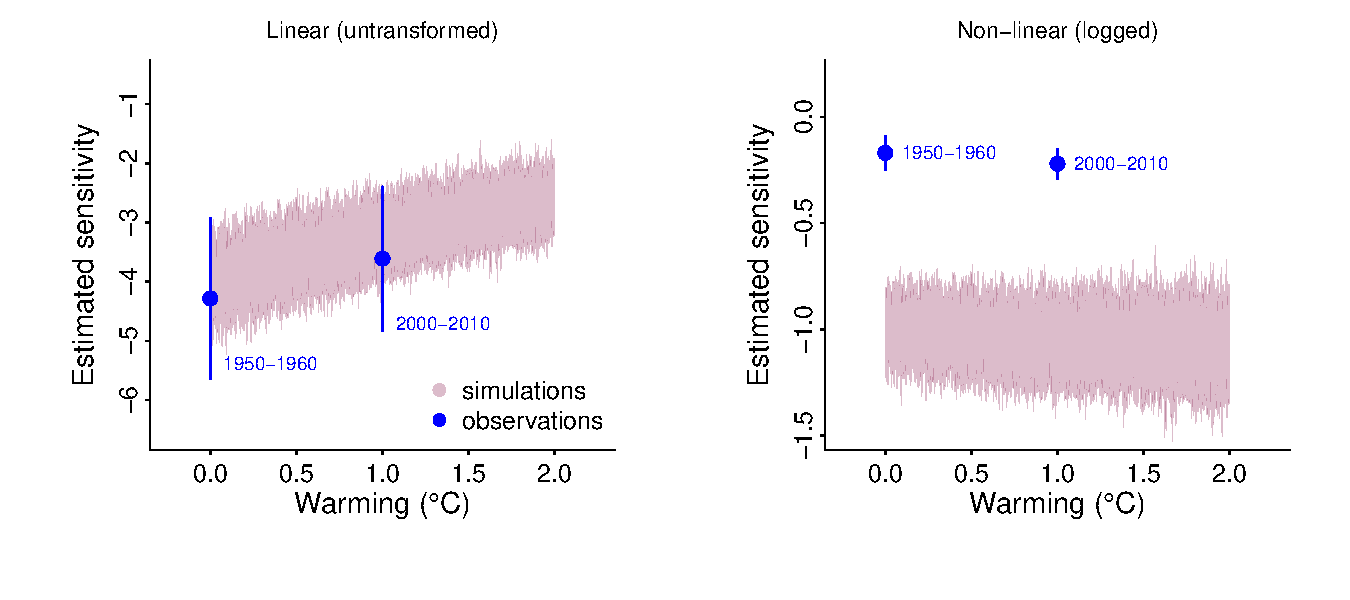
\includegraphics[width=1.05\textwidth]{..//analyses/figures/basicsimsandpepalt1.pdf} % 136 words
\caption{\textbf{Shifts in temperature sensitivities (response per $^{\circ}$C)  with warming occur when using linear models for non-linear processes.} Estimated sensitivities decline with warming in simulations (shading, estimated across 45 sites with a base temperature of normal(6,4), variation comes from fluctuation in the Monte Carlo simulations) with no underlying change in the biological process when sensitivities were estimated with linear regression (left). This decline disappears when performing the regression on logged predictor and response variables (right). Such issues may underlie declining sensitivities calculated from observational data, including long-term observations of leafout across Europe (for \emph{Betula pendula} from PEP725 from for the 45 sites that had complete data for 1950-1960 and 2000-2010), which show a lower sensitivity with warming when calculated on raw data, but no change in sensitivity using logged data. Shading, symbols and lines represent means $\pm$ standard deviations of regressions across sites. See Supplementary Information for a discussion of why estimated sensitivities are -1 or lower in non-linear models.} % Estimates of sensitivities from logged variables were generally much lower than -1, suggesting other factors or a better metric of temperature underlie leafout dates.
\label{fig:basicsimswpep} % decsensSims.R
\end{figure}

\clearpage
\nolinenumbers
\setstretch{1.1}
\section{Letter}
Editor and reviewer comments are in \emph{italics}, while our responses are in regular text. \\ % and all in-text citations generally cross-reference to the main text.

{\bf Editor's comments:} \\

\emph{You'll see that while two of the reviewers (#1 and #3) are convinced by your study, the other two still need more clarity and detail to persuade them.}\\

We thank the editor for the opportunity to revise our manuscript. We found the reviewers comments very helpful, with many overlapping requests for clarity or a more careful message. We provide detailed point-by-point responses below.\\

{\bf Reviewer 1 (A Donnelly) comments:} \\

\emph{The authors present a very interesting and important analysis to demonstrate how a decline in temperature sensitivity with warming is obtained using linear regression but the decline disappears when both variables (temperature and leafout dates) are log transformed. This is a very important and timely finding which has implications for future predictions of the impact of climate change on phenology. I would expect this report to motivate researchers to re-examine trends in phenology using this method. The manuscript is extremely well written, explained and presented. Therefore, I recommend this short report for publications without revision.}\\

We thank the reviewer for the positive comments on the manuscript's topic and writing style. We have worked to maintain these good aspects of the manuscript while addressing other reviewer comments. \\

{\bf Reviewer 2 comments:} \\

\emph{This MS provides a simple explanation for the observed non-linearity in biological temperature sensitivity (the observation that at higher temperatures the biological temperature sensitivity per degree Centigrade is decreasing): non-linearity in the biological temperature response. The MS develops a model to prove this point and it is very nicely written. Nevertheless, I found this somewhat uncompelling, because that the explanation appears to be the same as the observation (e.g. crows are black, because crows are black). The main problem appears to be a criticism in how words are used in temporal ecology literature: ``sensitivity'' versus ``response''. Indeed, many authors have used the word ``(in)sensitivity'' rather than the word ``response'' and this could be criticized, because ``(in)sensitivity'' implies some fundamental shift in the temperature response mechanism, even though what we are really seeing is an unchanged response. However, taking this into account the MS is reduced to a semantic discussion, in that not the sensitivity but the response is non-linear.}\\

We understand the reviewer's concerns to be that our finding may seem obvious to some, but we don't see it as a purely semantics debate for several reasons. First, there is a growing use of shifting or declining sensitivities as evidence of shifts in the underlying biology in the climate change literature, without a robust interrogation of whether this evidence supports the underlying hypothesis. Second, other reviewers of this manuscript here, and additional reviews we gathered from researchers in the field suggest the main crux of our manuscript (that temperature responses are non-linear and thus linear models used to estimate those responses will find declining sensitivities with warming temperatures) was surprising to them. We ourselves were surprised by this result and did not find it intuitive. Third, our simulations show that many models expected to produce declining sensitivities do not (we discuss this more in the following comment), and thus show how critical developing more robust expectations in this area of research may be to progress. Thus, while we understand our findings may not be surprising to some in the field we believe they are novel to many and that highlighting the statistical issue and providing a theoretical underpinning to explain it is an important and useful advance.\\

\emph{Either way, if temperature becomes a non-limiting factor with warming, other environmental factors will inadvertently take over, changing selective pressures on organisms. Therefore, I also do not see how this simple explanation for non-linearity of temperature sensitivity could discredit the conclusion that fundamental aspects of biological processes are being reshaped by climate warming, as the abstract appears to suggest.}\\

We agree with the reviewer that our model does not refute that shifting biological processes could underlie observations of declining sensitivities, and we did not mean to suggest otherwise. We fully agree that with continued warming, we should expect a greater role of factors beyond spring temperatures, but we believe our results highlight that most current methods may not capture this well. To address this we have: (1) adjusted our language in the abstract, which we now close with ``Current methods may thus undermine efforts to identify when and how warming will reshape biological processes'' and in the main text, \lr{R2biomattersstart}-\lr{R2biomattersend}:
\begin{quote}
Our results do not rule out that important shifts in biological processes may underlie observations of declining temperature sensitivities, but provide a simpler explanation for them. Instead, our results highlight how the use of linear models may make identifying when (and potentially why) warming alters underlying biology far more difficult.
\end{quote}
(2) We have provided a longer discussion of the expectation that other environmental factors should play a larger role with warming in the main text (\lr{biomattersstart}-\lr{biomattersend}). (3) We have included an extended discussion and analyses of alternative models in the supplement (see new sections `Effect of shifting $\beta$ on sensitivity' and `Simulations of common hypotheses for declining sensitivity'). In our previous draft we provided a simulation where reduced overwinter chilling led to a greater thermal sum requirement with warming, we now explain this simulation in more detail. Interestingly, this simulation does not always produce declining sensitivities---for example, we now show in `Effect of shifting $\beta$ on sensitivity' that increasing the thermal sum for leafout would produce \emph{increasing} (i.e., more negative) sensitivities estimated from linear models and the exact predictions for how sensitivities should shift with climate change depend strongly on the underlying model of chilling, forcing and how warming co-varies with each. We now also provide one photoperiod simulation as well, which also highlights the complexity of teasing out other cues. While the focus of our manuscript remains on the statistical issue of using linear models for non-linear temperature processes with warming---which extends beyond spring plant phenology---we hope these examples better highlight the challenges of modeling these processes with current data and show that our assumptions from verbal models may not always be accurate. \\

\emph{The MS could narrow its focus to just being about the difference between ``sensitivity'' and ``response'' to temperature, and that it is important to provide accurate definitions. Moreover, it could urge the field not to overreach in their conclusions on biological temperature responses.}\\

We agree and have worked to balance the manuscript better to contrast our findings with biological expectations given warming, and how well we can detect them. We have also reviewed our uses of the terms, `sensitivity' and `response' for accuracy and clarity; for example, see changes on \lr{semantic1}, \lr{semantic2}, \lr{semantic3} and in main text figure caption.\\

\emph{On a different note, the number of citations is inadequate. For example, on p4 paragraph 1 is the first mention of "thermal sum" without any citation. This happens more often, and should be revised thoroughly.}\\

Our updated manuscript includes 13 additional citations (our original draft included 12), see in particular \lr{addcites1}, \lr{addcites2}, \lr{addcites3}. \\% 12 refs originally
%``The 'heat unit approach," in use for over two centuries, is a scheme for studying plant-temperature relationships by the accumulation of daily mean temperatures above a certain threshold temperature during the growing season'' from \citep{wang1960}\\

\emph{I have no small textual comment, as the MS is very well written.}\\


{\bf Reviewer 3 (CM Zohner) comments:} \\

\emph{I really like this study. It is an important warning to phenologists that the commonly-used temperature sensitivity metric can be dangerously misleading. The modeling part makes sense to me but I wonder whether more information is required at some parts to allow readers to fully grasp what was done here. For instance, it is not totally clear to me how the PEP data was analysed. How did you determine the preseason lengths (which of course are also problematic per se) on which temperature sensitivities are ultimately based on? I recognize that this is a short report that does not allow for too many details but I think that the Supplementary part should still contain all necessary information to fully understand what has been done here.}\\

We are glad to hear the reviewer appreciated our manuscript and agree we could do more to make our methods clearer. We have updated our supplemental section, `Methods \& results using long-term empirical data (PEP725)' to better explain our methods. We used pre-defined pre-seasons; we are now more explicit about this and for transparent provided two shorter pre-season windows (see updated tables \ref{tab:pep10yr}-\ref{tab:pep20yr}). The relevant text now reads:
\begin{quote}
To examine how estimated sensitivities shift over time, we selected sites of two common European tree species (silver birch, \emph{Betula pendula}, and European beech, \emph{Fagus sylvatica}) that have long-term observational data of leafout, through the Pan European Phenology Project \citep[PEP725,][]{Templ2018}. We selected these two species given that they were best represented for consistent data at the same sites over our study years for an early-leafout (\emph{Betula pendula}) and a late-leafout (\emph{Fagus sylvatica}) species (e.g., \emph{Betula pendula} had 17 sites with leafout data from 1950-1960 and 2000-2010, while the next best option for an early-leafout species, \emph{Alnus glutinosa}, had data for only five sites). We used sites with complete leafout data across both our 10-year (and 20-year) windows to avoid possible confounding effects of shifting sites over time (see Tables \ref{tab:pep10yr}-\ref{tab:pep20yr} for numbers of sites per species x window). \\

To calculate temperature sensitivities, we used a European-wide gridded climate dataset \emph{\citep[{\normalfont E-OBS},][]{cornes2018}} to extract daily minimum and maximum temperature for the grid cells where observations of leafout for these two species were available (Fig. \ref{fig:pepdaily} shows a subset of the climate data for 14 sites used). Determining the appropriate window over which to estimate a temperature sensitivity for spring plant phenology is an area of active research \citep{gusewell2017,xupreseason2018}. Ideally researchers wish to separate windows over which chilling and forcing apply \citep[if they can be cleanly separated,][]{linkosala2008,lundell2020}, but this is generally impossible given our limited understanding of the two processes \citep{chuine2016}. Researchers thus either use a pre-defined spring window \citep[e.g.,][]{zhnag2015,park2018remsens,Park2019,kopp2020} or use a statistical search to determine window attributes; for example, some use a set period then search for a start date \citep[e.g.,][]{Cook:2012pnas,wang2015ecoind}, while others search for both a start date and window length \citep[e.g.,][]{fu2015,tansey2017}. Given the non-identifiability of the simple chilling + forcing model described above (`Simulations of common hypotheses for declining sensitivity'), we do not feel there is sufficient evidence that statistical searches for pre-season windows will select biologically relevant periods related to forcing, and more easily could add additional layers of non-identifiability (to date, most pre-season windows are fit as separate analyses making such issues harder for researchers to identify). Thus, we used pre-determined windows from 1 March to 30 April (60 d; we also present windows of 45 d, from 1 Mar to 15 Apr, and for 31 d, from 15 Mar to 15 Apr, for comparison). Our window represents a period in the spring when forcing is likely the dominant cue, and is similar to many other studies of temperature plants using pre-defined windows \citep[e.g.,][]{prevey2017,Park2019}. We then estimated the sensitivity as a simple linear regression of leafout day of year versus the mean daily temperature over the window (`slope' in Tables \ref{tab:pep10yr}-\ref{tab:pep20yr}), or a simple linear regression using logged versions of these predictors (`log-slope' in Tables \ref{tab:pep10yr}-\ref{tab:pep20yr}). \
\end{quote}

\emph{Additionally, I think it is important to emphasize in the text that, although the days per °C metric does not seem to be adequate to detect changes in the phenological responses to temperature, it is still likely that these changes are happening at the moment. You could for example cite some experimental studies, including your own meta-analysis of these studies, that clearly show that the required warming to leaf-out is increasing as winters become shorter, e.g., refs(1-4). The linear dashed line in Figure 3b in ref(5) also demonstrates that, while winter chilling and day length seem to have large effects on the amount of warming (degree-days) to leaf-out, the apparent temperature sensitivity doesn't really change, otherwise one should see a flattening curve. So, while I totally agree that the days per °C metric can be totally misleading, I think the paper would benefit from a short discussion on the importance of spring phenology drivers apart from spring temperature to
emphasize that they are important, although probably not directly visible in the days per °C metric.}\\

This is a good point and somewhat related to points raised by Reviewer \#2. To address it we have, (1) changed the ending the abstract to ``Current methods may thus undermine efforts to identify when and how warming will reshape biological processes,'' (2) provided a longer section in the manuscript, \lr{biomattersstart}-\lr{biomattersend}, which reads (and now cites most of the suggested citations):

\begin{quote}
Fundamentally rising temperature should alter many biological processes, making robust methods for identifying these changes critical. In spring plant phenology, where declining sensitivities are often reported \citep{fu2015,piao2017,dai2019ag}, warming may increase the role of `chilling' (determined mainly by winter temperatures) and daylength \citep{Laube:2014a,zohner2016}---potentially increasing the thermal sum required for leafout at lower values of these cues \citep{Polgar2014,zohner2017,flynn2018}. Adjusting our simulations to match this model yielded shifts in sensitivities with warming. Unlike a model with no underlying biological change, however, after correcting for non-linearity the shifts in sensitivities remained and they occurred in step with the biological change (Fig. \ref{fig:simsshiftcues}a, c). In contrast, sensitivities estimated from a linear model showed shifts across the entire range of warming, well before the simulated biological change (Fig. \ref{fig:simsshiftcues}a, c). Further, we found that an increase in the thermal sum required for leafout should yield larger temperature sensitivities, not smaller, as often expected \citep[e.g.,][]{fu2015}, thus highlighting the complexity of what trends to expect in sensitivities with warming (see `Common hypotheses for declining sensitivity' in Supplementary Information for an extended discussion).
\end{quote}

\emph{References}\\
\emph{1. 	J. Laube, T. H. Sparks, N. Estrella, J. Höfler, D. P. Ankerst, A. Menzel, Chilling outweighs photoperiod in preventing precocious spring development. Glob. Chang. Biol. 20, 170-182 (2014).}\\
\emph{2. 	C. Polgar, A. Gallinat, R. B. Primack, Drivers of leaf-out phenology and their implications for species invasions: Insights from Thoreau's Concord. New Phytol. 202, 106-115 (2014).}\\
\emph{3. 	C. M. Zohner, B. M. Benito, J. D. Fridley, J. C. Svenning, S. S. Renner, Spring predictability explains different leaf-out strategies in the woody floras of North America, Europe and East Asia. Ecol. Lett. 20, 452-460 (2017).}\\
\emph{4. 	D. F. B. Flynn, E. M. Wolkovich, Temperature and photoperiod drive spring phenology across all species in a temperate forest community. New Phytol. 219, 1353-1362 (2018).}\\
\emph{5. 	C. M. Zohner, L. Mo, T. A. M. Pugh, J. F. Bastin, T. W. Crowther, Interactive climate factors restrict future increases in spring productivity of temperate and boreal trees. Glob. Chang. Biol. 26, 4042-4055 (2020).}\\


{\bf Reviewer 4 comments:} \\

\emph{In this short manuscript, the authors intended to show that rising temperatures combined with linear estimates based on calendar time are expected to produce observations of declining sensitivity without any shift in the underlying biology. While the topic is very interesting and the conclusion is eye-catching, I found that the reasoning and presentation of the manuscript deserved much more reconsideration and the conclusions were not convincing.}\\

\emph{My general feeling is that the manuscript was presented in a form that was very hard to follow. For example, the authors presented a stochastic experiment, whose details were buried in the supplementary information. Many critical details of the experiments were missing, making it difficult to assess. The authors later argued a ``correction'' for non-linearity, but the theorem of this correction and its caveats were not presented. Coming after that, the authors intended to test their theory with the observation dataset (PEP725), but critical details on how they calculated the temperature sensitivity was not clear, which, as Keenan et al. (2020) mention, is a fundamental issue in deriving temperature sensitivity. I have to read the short manuscript for several times, tracing backward and forward between the main-text and SI, and taking some guesses to what they have done. Thus, I strongly recommend the authors to make a full-length paper with clear presentation on their methods
and reasoning. In its current form, the manuscript is not publishable in my opinion.}\\

We appreciate the reviewers concerns that we should have provided more clear methods for our PEP725 analyses, and this was also a concern of Reviewer 3. To address this we have greatly extended the section in the supplement on the PEP725 analysis, providing full methods (see also the response above to Reviewer 3's first point, where we show much of the relevant text). \\

Our stochastic experiment is designed to be simple---a model where an event is triggered based on a thermal sum threshold, as we describe in the main text. We fully describe the stochastic model both mathematically and in a longer text format in the supplement. The correction we suggest (log transformation) is the natural transformation for an inverse relationship (by definition a log linearizes this relationship) so we are unsure how to further describe this. While we could move the mathematical description of the model into the main text, we feel that will narrow the readership unnecessarily---as the model is fundamentally very simple and already described in the main text. We provide the supplement math as a more developed proof for those interested. Based on several reviews by those in this research area, including those of the other three reviewers here, we believe this format of the manuscript allows readers to understand our main point, analyses and findings.\\

\emph{A major argument made by the authors was a stochastic experiment: when leafout date was determined by a constant cumulative daily temperature, a declining apparent temperature sensitivity could be derived. However, this argument has two limitations: (1) the assumption of constant threshold of cumulative heat is a very strong one, and not supported by observations (e.g. Fu et al., 2014); (2) even we accepted the strong assumption, it does not prove that the observed decline in apparent temperature sensitivity comes from unchanged heat accumulation. As the authors showed, increasing heat requirements could indeed yield declining apparent temperature sensitivity. As a reader, I do not see the value of this stochastic experiment, which did not successfully prove the points made by the author. }\\

We did not mean to suggest that our model proves declining sensitivities are driven by the model we present and we should have made this clearer. As noted above in our reply to Reviewer 2, to address this we have: (1) adjusted our language in the abstract, which we now close with ``Current methods may thus undermine efforts to identify when and how warming will reshape biological processes'' and in the main text, \lr{R2biomattersstart}-\lr{R2biomattersend}:
\begin{quote}
Our results do not rule out that important shifts in biological processes may underlie observations of declining temperature sensitivities, but provide a simpler explanation for them. Importantly, our results highlight how the use of linear models may make identifying when (and potentially why) warming alters underlying biology far more difficult.
\end{quote}
Regarding the assumption of the constant threshold of cumulative heat, we have added a new section (`Effect of shifting $\beta$ on sensitivity') that examines the effects of relaxing this assumption and find that, perhaps contrary to expectations, an shifting thermal sum would produce increasing, not declining sensitivities. We did not include this before as we aimed to test a simple model so that we could understand expected shifts in sensitivities without this effect. We are not aware of strong observational evidence that this threshold is varying (Fu \emph{et al.} 2014 in \emph{PLOS One} and Fu \emph{et al.} 2015 in \emph{Nature} both use methods similar to the we critique here to suggests shifting thresholds, but we may be reviewing the wrong papers), though we now clearly state and cite experimental evidence that these thresholds can shift (\lr{biomattersstart}-\lr{R4end}):
\begin{quote}
Fundamentally rising temperature should alter many biological processes, making robust methods for identifying these changes critical. In spring plant phenology, where declining sensitivities are often reported \citep{fu2015,piao2017,dai2019ag}, warming may increase the role of `chilling' (determined mainly by winter temperatures) and daylength \citep{Laube:2014a,zohner2016}---potentially increasing the thermal sum required for leafout at lower values of these cues \citep{Polgar2014,zohner2017,flynn2018}.
\end{quote} 
In addressing concerns from Reviewers 2-3, we also provide an extended discussion of the complexity of outcomes from models that predicting shifting thermal sums based on other cues for spring phenological events. While many of the authors ourselves assumed that sensitivities to spring temperatures should decline as other cues come into play, this is not always the case given the co-variation of many of these cues, and highlights the value of explicit models to challenge assumptions. \\

\emph{In the next paragraph, the authors argued that a log transformation could make the declining temperature sensitivity disappear. While this may be true, an issue may arise as the log transform would make the regression sensitive to a few outliers and it will necessarily hide change in temperature sensitivity, if it happens. So I hardly see how the disappearance of linearity after log-transformation proves that non-linearity did not exist in the observations.}\\

Log transformations make regressions less (not more) sensitive to outliers, which we assume is what the reviewer means, though we're not clear if the concern here is regarding outliers in the predictor or response, or both. Our argument is that a log is the correct transformation for the data given the model that plants leafout after reaching a threshold thermal sum. As mentioned above, we do not mean to suggest that our model in any way proves that there are not biological shifts underlying the PEP 725 data, but that our current statistical methods may not be robust to detecting to these changes, and we have edited the abstract and main text to clarify this. \\

\emph{Also about the analyses on the observation dataset: the PEP dataset includes much more species than the two used here, why selectively analyzing these two species?}\\

Good catch, we now clarify our methods regarding species selection in the supplement (`Methods \& results using long-term empirical data (PEP725)'). We write:
\begin{quote}
 We selected these two species given that they were best represented for consistent data at the same sites over our study years for an early-leafout (\emph{Betula pendula}) and a late-leafout (\emph{Fagus sylvatica}) species (e.g., \emph{Betula pendula} had 17 sites with leafout data from 1950-1960 and 2000-2010, while the next best option for an early-leafout species, \emph{Alnus glutinosa}, had data for only five sites). 
\end{quote}
For clarity we provide on the following pages the number of sites for other major species in the PEP725 data, including our analyses of the species with the third most data for our analyses, \emph{Quercus robur}.\\

\emph{Overall, the stochastic experiment showed that declining apparent temperature sensitivity could have some alternative explanation, but it is far from sufficient to conclude that the observed declining temperature sensitivity was from the authors' assumption. The empirical analyses were not performed in a transparent and convincing way. Therefore, I could not draw similar conclusions as the authors did.}\\

Our goal with the stochastic experiment was to show, as this reviewer writes, ``that declining apparent temperature sensitivity could have some alternative explanation,'' and thus we believe our manuscript, on some level, did communicate our main finding. We have worked to adjust our language to make it clear we do not mean to state that we have shown this is the definitive explanation, but instead that it is an explanation that should be better considered in analyses using declining sensitivities with warming as evidence of shifting biology with warming. We believe our revisions have further clarified our methods, analyses and conclusions and thank the reviewer for this.



\end{document}




\section{Outline \& notes}

Need to work on this, notes to date on % \href{https://github.com/lizzieinvancouver/decsens/wiki/Statistical-artifacts-in-sensitivities}{here}.\\

\emph{Meeting with Jonathan Auerbach \& Andrew Gelman on 18 December 2019:} 

Fundamental issue is that we have a non-linear relationship ($y=1/x$) being described by a linear function ($y=x$), where $x$ is the mean temp and 1 could be the GDD. The time until you reach a threshold is inversely proportional to the speed you go at. So, at very low temperatures plants would (theoretically) never leaf out and at 200 C days it would take one day. \\

The classic algebra example (they tell me) is how long does it take to drive 200 miles? It depends on your miles per hour. (Side note by Lizzie while typing up these notes: the speed analogy is sort of nice, climate change is stepping on the accelerator, making this algebra problem relevant.)

\begin{itemize}
\item The artifact comes from the mean getting larger while the variance goes down (I think, I may have this noted wrong, but it's about the mean relative to the variance, not just the variance or the mean). If you make the variance scale with the mean you will see the issue go away (though Andrew pointed out this should be done on the $SD$ scale, not the $var$).
\item ``The statistical artifact is that fitting a linear regression requires linearity''said  Jonathan Auerbach.
\item If this was all simple, we could fix it two ways: percent scale (decline relative to some base C temp) or log both axes. (Note from Lizzie: but we don't know when to start accumulating so not sure how this works, though Jonathan seemed to have insight into this.)
\item An example of inferring process from an artifact is regression to the mean, though Andrew pointed out regression to the mean is more complicated compared to this as regression to the mean is a statistical issue and this is just a deterministic reality. 
\item Convexity in economics has had similar problems to this. 
\end{itemize}

\section{Literature notes}

Sagarin 2001: False estimates of the advance of spring (leap year issues). \\

I noticed as you go back to 2014 and before in my ISI searches, you get a lot of soil respiration lit. And in that literature they use $Q_{10}$ for temperature sensitivities, ``[t]he temperature sensitivity of soil respiration is often expressed as the Q10 value; that is, the factor by which soil respiration increases by a 10°C increase in temperature (e.g., Kirschbaum, 1995; Van't Hoff, 1898),'' which would avoid a good dose of the issue we're seeing.\\  % definition from https://agupubs.onlinelibrary.wiley.com/doi/full/10.1002/2017GB005644
% Van't Hoff, J. H. (1898). Lectures on theoretical and physical chemistry. In Chemical Dynamics Part I (pp. 224–229). London: Edward Arnold.

Shen et al. 2014 shows earlier-season vegetation more temperature-sensitive, which is the same artifact. Do we want to work this in?
